\chapter{Interface do Usuário}\label{cha:interface}
\begin{figure}[h]
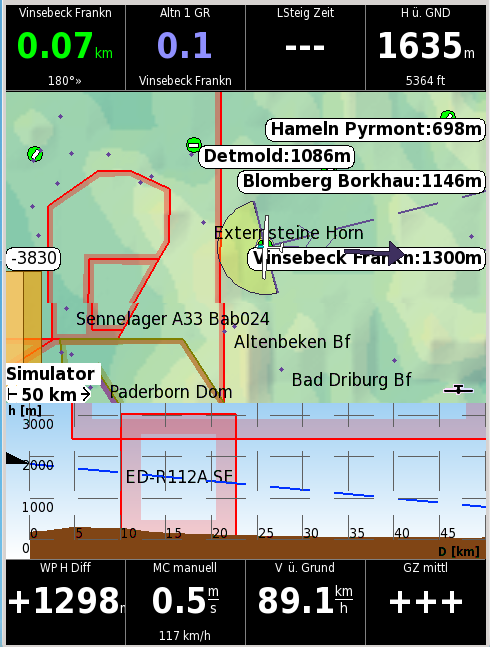
\includegraphics[angle=0,width=\linewidth,keepaspectratio='true']{figures/plain.png}
\caption{Layout mais comum da tela do XCSoar}
\end{figure}

Este capítulo descreve de um modo geral, os conceitos fundamentais da interface do usuário usados pelo XCSoar.  A tela principal mostra a maioria das informações necessárias para o vôo normal.   Geralmente a tela principal é composta de um mapa móvel e infoboxes.  Por várias razões – não é o escopo da introdução – você tem a oportunidade de utilizar várias telas principais, chamadas de páginas de telas.

As páginas de telas são facilmente acessadas por um gesto de deslizamento horizontal, como se tivesse virando páginas de um livro ou por um apertar de botão, dependendo do hardware que estiver usando.  Com a página de telas você estará apto a compor várias telas principais para tirar vantagem da sua utilização em diversas situações de vôo.  Simplificando, você poderá usar a informação apropriada em diferentes casos, podem ser acessadas muito facilmente e rapidamente.

Sempre que alguma situação que pode tirar a atenção do piloto, é mostrada uma informação na tela principal.  Isto acontece especialmente quando há a necessidade de reação do piloto, como uma possível colisão ou quando o piloto irá entrar em uma área de espaço aéreo restrito.

Evidentemente, os botões de menu e menu de telas também são sobrepostos à tela principal.  Como resultado, os elementos apresentados sobrepostos formam uma pilha de exibição com a tela principal representando a base.  As descrições mais detalhadas serão apresentadas nos capítulos seguintes. 


\section{Elementos exibidos}
\subsection*{Tela principal e página de telas}
Cada página de tela do conjunto de páginas do XCSoar é composta de várias partes:

\begin{description}
\item[Área principal] a grande parte da tela é normalmente dedicada à movimentação do mapa do GPS.  Vários símbolos relativos à informação de vôo são sobrepostas ao mapa.  Os ícones e textos devem aparecer ao longo da borda inferior da tela para indicar o estado dos dispositivos conectados, modos de vôo, etc.  De acordo com a evolução do desenvolvimento do XCSoar, há um aumento do número de itens que podem ser escolhidos para serem mostrados na área principal, como medidores FLARM, Radar, Assistente de Termal e Horizonte (como na versão 6.7.2, Dez. 2013).

\item[InfoBoxes] Uma grade de dados é mostrada na parte superior e inferior da tela (formato de retrato da tela), ou do lado direito da tela (formato de paisagem da tela).  São chamados de dados de infoboxes do GPS e outros dispositivos de entrada, bem como podem ter cálculos efetuados pelo XCSoar. Além disso, as Infoboxes podem mostrar também medidores e alguns gráficos.
\end{description}

\subsection*{Sobreposições}
\begin{description}
\item[Instrumentos]  os instrumentos mostram as medições dos sensores.  Todos os instrumentos são opcionais e alguns só poderão mostrar seus dados quando conectados aos dispositivos externos.  A sobreposição do instrumento na tela principal é permanentemente mostrada ou é somente mostrada em algumas condições críticas.  Ex. o assistente de termal é mostrado somente quando o XCSoar entra em modo de giro.  O radar FLARM é mostrado toda vez que há a possibilidade de colisão.  Os instrumentos permanentemente mostrados são a barra de planeio final, bem como a barra de variômetro, entre outros.

\item[Rótulos de Botões e Menus] Os botões do dispositivo que está rodando o XCSoar podem ser usados para navegar em pequenos menus na tela e são normalmente sobrepostos aos menus e podem ser selecionados apertando o botão deste item.  Se o dispositivo possui tela de toque, o item de menu pode ser selecionado clicando sobre o mesmo.  Estes botões são desenhados com texto preto em fundo cinza. 

\item[Mensagem de condição (estado)]o texto é mostrado sobre a tela em uma caixa de mensagens.  Este texto é utilizado para mostrar informações detalhados ao piloto quando alguns eventos ocorrem.

\item[Janela de diálogo] uma grande janela de diálogo, normalmente contendo gráficos e botões são usadas para mostrar dados detalhados ao piloto, relativos aos detalhes de waypoints, estatísticas e análises, etc.

\item[Menu principal] O menu principal é acessado clicando duas vezes na área do mapa ou infoboxes, bem como também por gesto.  Se o menu de botões não for pressionado após algum tempo, desaparecerá da tela para não obstruir a área do mapa. 
\end{description}

\subsection*{Mostrador de vário clássico}
Como dito acima, os mostradores podem ser mostrados de formas diferentes, em infoboxes, sobrepostos ou mesmo na área principal.  O mostrador do variômetro tradicional é diferente.  O mostrador em estilo agulha é mostrado permanentemente, escolhendo o layout da infobox que inclui o variômetro do lado direito das outras infoboxes.

\section{Interação}
Existem várias maneiras de interagir com o XCSoar:
\begin{itemize}
\item Tocando certos elementos no mapa
\item Tocando nas infoboxes e nos botões dos menus da tela.
\item 'Gesticulando', como por exemplo, desenhando um traço da esquerda para a direita na tela (veja seção  \ref{sec:gestures} abaixo).
\item ‘Arrastando’ a tela (tocando a tela e movendo antes de soltar).
\item Apertando os botões de função do dispositivo.
\item Apertando as teclas de cursor do dispositivo.
\item Apertando teclas ou chaves em um dispositivo conectado ao XCSoar.
\end{itemize}

Dependendo do dispositivo conectado ao XCSoar, nenhum destes métodos de interação são possíveis e podem haver números diferentes de funções dos botões.

Para a versão do XCSoar para PC, clicar com o mouse sobre um item tem a equivalência de tocá-lo.

Como o Altair não tem uma tela de toque, todas as interações do usuário são feitas através de botões físicos, chaves ou outro dispositivo conectado.  


\section{O menu principal de botões}
O menu de botões é um conjunto de botões mostrado na tela e ativado por toque ou botões físicos (quando houver no dispositivo).  Esta é a forma primária de interagir com o XCSoar.

\subsection*{A interface básica}
O menu é organizado em quatro grupos diferentes de funções, geralmente em forma de hierarquia.  O layout do menu depende da configuração de botões do hardware e plataforma, e podem também serem personalizados pelo usuário.

O XCSoar pode também aceitar entradas de teclados externos, gamepads, joysticks, etc.  Podem ser atribuídas às estas entradas uma grande variedade de funções.
\sketch{figures/buttonmenu.png}
Para o Altair, há quatro menus principais, ativados por um dos botões físicos verticais do lado esquerdo da tela.  Quando um menu é ativado, uma faixa de botões aparece na parte inferior da tela.  Apertando um botão do menu específico da tecla, irá entrar em várias páginas deste item.  Apertando o botão horizontal correspondente irá ativar o item.  Na última página, apertando o botão de menu novamente, irá desativar este menu e a faixa apresentada na tela desaparece.
Para a versão de PC, estes botões de modo são ativados pelas teclas 1, 2, 3 e 4.  As teclas 6, 7, 8, 9 e 0 correspondem à faixa horizontal de botões.

Na versão PDA, os botões de modo são ativados pelas teclas laterais do joystick.

Se o usuário não interagir com o computador por algum tempo, o menu será fechado automaticamente.  Seu tempo para fechamento é configurável.  A tecla “ESC” no PC ou PWR/ESC no Altair também pode ser utilizada para fechar o menu.

O menu de botões aparece acinzentado se a função correspondente não está disponível.  Por exemplo, se a lista de waypoints aparecer cinza, não há waypoints carregados.
Vários rótulos de botões tem o texto dinâmico baseado em seu contexto, de modo a tornar mais claro o que acontecerá se o botão for pressionado.  A convenção é usada para descrever o que acontecerá se o botão for pressionado. Por exemplo, se o botão descrever \bmenug{MC Auto},portanto, apertando o botão irá deixar o “Auto MacCready” e o texto do botão irá indicar \bmenug{MC Manual}. 
Neste menu descrito acima, são utilizados os rótulos genéricos. 

\subsection*{Menu de funções de grupo}
Esta seção descreve o layout padrão do sistema de menus em todas as plataformas.  As funções desempenhadas por cada botão são descritas com mais detalhes nos capítulos seguintes.

Os botões primários são ativados pelos botões na faixa vertical no Altair, do topo para baixo:

\begin{jspecs}
\item[\bmenug{Nav}] Ações para controle de navegação, provas simples de vôos de cross-country.
\item[\bmenug{Mostrar}]Ações para controle da tela.
\item[\bmenug{Config}] Configuração do XCSoar, dispositivos conectados e ajustes de vôo.
\item[\bmenug{Info}] Ativa várias janelas de diálogo de informações.
\end{jspecs}

Na versão para PC, as teclas 1, 2 3 e 4 ativam os menus correspondentes.  A lista de menus seguinte tem somente o lado esquerdo da maioria dos menus de botões e suas respectivas seções.  Siga-os para verificar todos os detalhes de cada um.

\section{Visão geral do Menu}

\subsection*{Menu de navegação}
\noindent\makebox[\textwidth]{%

\begin{tabularx}{1.44\textwidth}{c|ccccc}
\bmenus{Nav 1/2}
 & \bmenus{Prova}
 & \bmenut{Pto. virada}{Anterior}
 & \bmenut{Próx. Pto.}{Virada}
 & \bmenut{Lista}{Waypoint}
 & \bmenus{Alternativos} \\
veja
 & \ref{cha:tasks}
 & \ref{sec:advanc-rest-tasks}
 & \ref{sec:advanc-rest-tasks}
 & \ref{sec:waypoint-selector-dialog}
 & \ref{sec:alternates} \\ \\
\bmenus{Nav 2/2}
 & \bmenut{Prova}{Abortar}
 & \bmenut{Marcar}{Ponto}
 & \bmenus{Alvo}
 & {}
 & {} \\
veja
 & \ref{sec:taskabort}
 & \ref{sec:markers}
 & \ref{sec:waypointdetails}
\end{tabularx}}

Você não deve iniciar o uso do XCSoar sem antes saber sobre todas as características do “Alternativos”.  Qualquer “Prova” relacionada no menu de navegação é usada para planejar o vôo de cross-country e certamente será o segundo passo.

\subsection*{Menu Mostrar menu}
\noindent\makebox[\textwidth]{%

\begin{tabularx}{1.44\textwidth}{c|ccccc}
\bmenus{Mostrar 1/2}
 & \bmenut{Zoom}{In}
 & \bmenut{Zoom}{Out}
 & \bmenut{Zoom}{Auto}
 & \bmenut{Info}{Auto/...}
 & \bmenut{Pan}{On} \\
veja
 & \ref{sec:zooming}
 & \ref{sec:zooming}
 & \ref{sec:zooming}
 & \ref{sec:screenpages}
 & \ref{sec:panning} \\ \\
\bmenus{Mostrar 2/2}
 & \bmenut{Rótulos}{All/...}
 & \bmenut{Trilha}{Completo/...}
 & \bmenut{Terreno}{Desligado/...}
 & \bmenut{Topo.}{Desligado/...}
 & \bmenut{Espaço Aéreo}{Desligado/...} \\
veja
 & \ref{sec:maplabels}
 & \ref{sec:trail}
 & \ref{sec:terrain_topo}
 & \ref{sec:terrain_topo}
 & \ref{sec:terrain_topo}
\end{tabularx}}

A maioria dos menus mostrados estão disponíveis também com gestos ou atalhos do seu dispositivo.  Assim que estiver mais familiarizado om o XCSoar, provavelmente irá utilizar estes menus com mais freqüência. 

\subsection*{Menus de Configuração}
\noindent\makebox[\textwidth]{%

\begin{tabularx}{1.44\textwidth}{c|ccccc}
\bmenus{Config 1/3}
 & \bmenut{MacCready}{$+$}
 & \bmenut{MacCready}{$-$}
 & \bmenut{MacCready}{Auto}
 & \bmenus{Flight}
 & \bmenus{Vento} \\
veja
 & \ref{sec:stf}
 & \ref{sec:stf}
 & \ref{sec:auto-maccready}
 & \ref{sec:flight-setup}
 & \ref{sec:wind-setup} \\ \\
\bmenus{Config 2/3} 
 & \bmenus{SISTEMA}
 & \bmenus{Planador}
 & \bmenus{Dispositivos}
 & \bmenut{File}{Manager}
 & \bmenus{Replay} \\
veja
 & \ref{cha:configuration}
 & \ref{sec:glidepolar}
 & \ref{conf:comdevices}
 & {}
 & \ref{sec:logger-replay} \\ \\
\bmenus{Config 3/3} 
 & \bmenut{Registrador}{Iniciar}
 & \bmenus{Logar NMEA}
 & \bmenus{Espaço Aéreo}
 & \bmenus{Vega}
 & \bmenus{Profiles} \\
veja
 & \ref{sec:logger}
 & \ref{sec:raw-logger}
 & \ref{sec:airspace-filter}
 & {}
 & {}
\end{tabularx}}

O menu de configuração é geralmente parte da interação básica com o XCSoar.  Você não espera perder muito tempo em vôo fazendo ajustes na configuração, com exceção de ajustes de vento ou MacCready.  O item “Vega” fornece controle sobre o variômetro inteligente Vega.  Abrirá um sub-menu.


\subsection*{Menus de Informação}
\noindent\makebox[\textwidth]{%

\begin{tabularx}{1.44\textwidth}{c|ccccc}
\bmenus{Info 1/3}
 & \bmenut{FLARM}{Radar}
 & \bmenut{METAR}{TAF}
 & \bmenut{Oque}{aqui?}
 & \bmenut{Check}{list}
 & \bmenus{Análise} \\
veja
 & \ref{sec:flarm-traffic}
 & \ref{sec:metar-taf}
 & {}
 & \ref{sec:checklist}
 & \ref{sec:analysis-climb} \\ \\
\bmenus{Info 2/3}
 & \bmenus{Estado}
 & \bmenus{Meteoro}
 & \bmenut{Time}{Código}
 & \bmenut{Traffic}{List}
 & \bmenut{Assistente}{Termal} \\
veja
 & \ref{sec:flight-status}
 & \ref{sec:weather-forecast}
 & \ref{sec:team-flying}
 & {}
 & \ref{sec:thermal-assistant} \\ \\
\bmenus{Info 3/3}
 & \bmenus{Credits}
 & \bmenus{Espaços} {Aéreos}
 & \bmenut{Message}{Repeat}
 & {}
 & {} \\
veja
 & \ref{sec:credits}
 & 
 & 
 & 
 &
\end{tabularx}}

O Menu de Informações é sempre um bom referencial, quando não é uma boa dica para ajustar o MacCready, é uma ajuda mais elaborada em um escopo maior para decisões táticas sempre que for necessário para seu vôo.


\subsection*{O Sub-menu de Configuração do Variômetro Vega}
\noindent\makebox[\textwidth]{%

\begin{tabularx}{1.44\textwidth}{c|ccccc}
\bmenus{Vega 1}
 & \bmenut{Airframe}{Switches}
 & \bmenut{Setup}{Audio}
 & \bmenut{Manual}{Demo}
 & \bmenut{Setup}{Stall}
 & \bmenus{Accel} \\ \\
\bmenus{Vega 2}
 & \bmenut{ASI}{Zero}
 & \bmenut{Accel}{Zero}
 & \bmenus{Store}
 & \bmenut{Cruise}{Demo}
 & \bmenut{Climb}{Demo}
\end{tabularx}}

As funções deste sub-menu requerem o variômetro inteligente Vega.  O menu pode ser acessado somente se o ‘Veja” for selecionado como dispositivo conectado.

\subsection*{O modo panorâmico do sub-menu do Menu Mostrar}

\noindent\makebox[\textwidth]{%

\begin{tabularx}{1.44\textwidth}{c|ccccc}
\bmenus{Pan}
 & \bmenut{Pan}{Off}
 & \bmenut{Zoom}{in}
 & \bmenut{Zoom}{out}
 & \bmenut{Oque}{aqui?}
 & {} \\
see
 & \ref{sec:panning}
 & {}
 & {}
 & {}
 & {}
\end{tabularx}}

Este sub-menu infelizmente se sobrepõe à tela principal no modo Panorâmico.  Suas funções são evidentes, todavia o menu pode ser reposicionado por tecnologia multi-toque ou botões (como no Altair).  Porém, juntamente com o botão “Pan Off” também há o botão “O que aqui?” que oferece um ótimo acesso à variedade de informações do mapa.

\section{Botões de Menu padrões}

Quando não há menu ativo (chamado de modo padrão), uma linha de botões no Altair desempenha as seguintes funções (da esquerda para a direita):

\begin{center}
\begin{tabular}{c c c c c c}
 PC: & 6 & 7 & 8 & 9 & 0 \\
 Altair: & F5 & F6 & F7 & F8 & F9 \\
& \bmenus{Voo} & \bmenut{Gerenciador}{Tarefas} & {} & \bmenus{Alvo} & \bmenut{Marcar}{Ponto} \\
\end{tabular}	
\end{center}

Teclando ESC no Altair mostrará os rótulos destes botões.
Para outras versões no modo padrão, o cursor faz as seguintes funções:

\begin{jspecs}
\item[Tecla Acima] Zoom +
\item[Tecla Abaixo] Zoom -
\item[Tecla esquerda] Marcar ponto
\item[Tecla direita] alterna entre as infoboxes normais e auxiliares e tela cheia
\item[Enter] Limpa a mensagem de estado ou suprime o mostrador FLARM se estiver aberto e se nenhuma mensagem de alerta estiver ativa.  
\end{jspecs}

Para a versão Altair em modo padrão, o botão rotativo desempenha as seguintes funções:
\begin{jspecs}
\item[Botão rotativo externo sentido anti-horário] Zoom +
\item[Botão rotativo externo sentido horário] Zoom -
\item[Botão rotativo interno sentido anti-horário] (Sem função atribuída)
\item[Botão rotativo interno sentido horário] (Sem função atribuída)
\item[Aperta botão rotativo] Limpa a mensagem do estado ou alerta de espaço aéreo.
\end{jspecs}

Nos formulários de diálogo, o botão rotativo no Altair desempenha as seguintes funções:
\begin{jspecs}
\item[Botão rotativo externo sentido anti-horário] Cursor para cima
\item[Botão rotativo externo sentido horário] Cursor para baixo
\item[Botão rotativo interno sentido anti-horário] Cursor esquerdo
\item[Aperta botão rotativo] Cursor direito
\item[Aperta botão rotativo] Tecla Enter
\end{jspecs}

Para o Altair, os botões ao longo da borda da tela podem ser usados como formas alternativas de navegação nos diálogos.  A tecla F4 (diretamente acima do botão rotativo) pode ser usada com um ENTER alternativo (ao invés de pressionar o botão rotativo) nos diálogos.  As teclas F6 e F7 (à direita do botão rotativo) podem ser usadas para selecionar a próxima página ou a anterior nos diálogos multi-páginas.

\subsection*{Rótulos dinâmicos de menu}
Certos menus têm rótulos dinâmicos para tornarem mais claro o que ocorre quando um menu for selecionado.  Além disso, itens que não estão disponíveis estão acinzentados para indicar que esta seleção não terá efeito algum.

A convenção usada para rótulos dinâmicos de menus é para rótulos que mostram a ação que será desempenhada quando o item do menu for selecionado.  Por exemplo “Luzes Acessas” irá ligar as luzes e o menu aparecerá “Luzes Apagadas” que só se apagarão se o menu for pressionado.  Esta convenção é usada no também no XCSoar.

Uma seleção de teclas de menus dinâmicos é mostrada abaixo:

\begin{description}
\item[\bmenug{Próx. Pto. Virada}]  
 Se acinzentado, a prova foi limpa ou se o ponto ativo foi finalizado.  Se estiver ativo, é o ponto principal para o final, e estará indicando “Waypoint finish”.
\item[\bmenug{Pto. virada anterior}]  
  Acinzentado se a prova foi limpa, ou se o ponto ativo é o início (start) e não há mais pontos de início.  Se houver múltiplos pontos de início e o pilão é o “start”, então aparecerá descrito “Cycle Start” para permitir a seleção entre os vários pontos de início.  Se o pilão ativo é o primeiro ponto após o início, aparecerá descrito “Waypoint Start”. 
\item[\bmenug{Rótulos Todos}]  
 Desta forma irá mostrar todos os rótulos disponíveis no mapa.  Há mais opções de visualização que mostrarão um pequeno número de rótulos como “Rótulos Prova”, não poluindo demais a tela.
\item[\bmenug{Alvo}]  
  Acinzentado se a prova foi limpa ou a prova abortada.

\end{description}


\section{InfoBoxes e páginas de telas}\label{sec:infoboxandpages}

A informação indicada nos campos da infobox podem ser selecionadas em uma grande variedade de opções (listadas no Capítulo 12).  Estes campos podem também ser utilizados por exemplo, para ajustes de MacCready.

O número específico e layout da grade da infobox depende da orientação da tela e do tamanho da tela do dispositivo.
Para uma tela de 320x240 de um Pocket PC em modo retrato, há quatro Infoboxes acima e quatro abaixo da tela de mapa.

Um layout normal de paisagem tem 9 infoboxes e o mostrador do variômetro do lado direito da tela.  Para telas maiores, podemos ter até 24 infoboxes mostrados simultaneamente.
\sketch{figures/infoboxes.png}

Para se ganhar clareza, quanto menos infoboxes você escolher para serem visualizados, mais fácil será a leitura dos mesmos.  Por outro lado, há muitas e muitas opções de infoboxes que o piloto não rejeitaria.  A quantidade de números possíveis de opções para Infoboxes excede 100 opções.  Por este motivo que o XCSoar oferece duas maneiras de gerenciar ainda mais opções do que o número de infoboxes.

Dependendo do seu estado de vôo, quando estiver girando ou voando reto, você pode deixar o XCSoar alterar o conteúdo de cada infobox.  Como exemplo, você deve mudar a infobox que mostra a média de subida na termal enquanto está girando para uma infobox que lhe informe a velocidade quando estiver voando reto.  Esta mudança é derivada automaticamente entrando em diferentes modos de vôo (seja seção 6.1), executando a mudança para outra janela de infobox.

Mais ainda, você pode usar as páginas de tela para mudar o conteúdo da Infobox manualmente, assumindo diferentes conjuntos na infobox para páginas diferentes (veja a seção seguinte).

Para ter acesso à mudança automática de infobox de acordo com o tipo de vôo, deixe o XCSoar rodar um o conjunto pré-configurado da instalação.  Para ajustar sua própria versão de infoboxes, siga o procedimento:

\begin{description}
\item[Geometria da InfoBox] escolha o layout da infobox.  O layout básico é mantido através de qualquer mudança no vôo, influenciando somente o conteúdo da infobox.\config{interface-appearance}
\item[Escolha Infobox "Auto"] Configure pelo menos uma página de tela com a escolha de Infobox “Auto”.  Como pode ser visto na tela configuração correspondente, há mais páginas de telas pré-definida.  As demais não são necessárias para terem alternância automática. 
\item[Defina os conjuntos de ajustes da Infobox] Agrupe o conteúdo da infobox que deseja que seja mostrada em três páginas de infobox chamada de “Girando”, “Planeio” e “Planeio Final”, respectivamente.
\end{description}
 

 
\subsection*{Página de telas com diferentes conjuntos de infobox}\label{sec:screenpages}

O XCSoar permite que o piloto defina os vários conjuntos de infoboxes que forem apropriados para o vôo normal.  Assume girando, voando ou planeio final como normal, o XCSoar pode alterar as infobox correspondentes automaticamente.

Como pode imaginar, há inúmeros casos de conjuntos que podem ser mostrados.  Você pode ter até oito conjuntos de páginas de telas, refletindo a situação atual.  Algumas possibilidades são dadas, só para fazer um breve resumo do uso do conceito da página de telas.

\label{par:use_case}
\begin{description}
\item[Familiarização] se você é um piloto de ponta, você está procurando obter os benefícios dos inúmeros cálculos e provas que o XCSoar pode fornecer.  Para ter estes benefícios relacionado às fases da competição, deve aceitar a idéia de definir dois casos especiais de páginas, para a fase de início, outra para a prova.  Se você procura por um valor específico para ser mostrado, vá ao Capítulo  \ref{cha:infobox} "Referências das Infoboxes". 
Há grande chance de achar lá.
\item[No chão] Como um gerenciador, você deve usar uma página de tela mostrando o “Radar FLARM” somente.  Pode acontecer na tela do PC rodando o XCSoar conectado a um receptor FLARM.
\end{description}

O que quer que seja que gostaria de mostrar, leve em conta o momento de uso e o conceito de página de telas.

\gesturespec{left}
Para ir através de várias páginas de telas, use as teclas esquerda/direita (Altair) ou gestos esquerda/direita (tela de toque) através do botão de menu \bmenug{Mostrar 1/2}, mostrando um rótulo dinâmico, mudando de acordo com o conteúdo da página de tela para mostrar o próximo:
\gesturespec{right}

\bmenut{Mostrar}{1/2}\blink\bmenut{Assistente de}{Térmica}\blink\bmenut{Info}{Planeio}\blink\bmenut{Info Planeio}{Final}\blink\bmenut{Info}{...}


\subsection*{Modificando o conteúdo da InfoBox }

(Esta seção somente se aplica se houver tela de toque ou mouse presente).  Alguns valores de infobox podem ser alterados pelo usuário selecionando (ex. longo pressionamento) o dado no infobox na tela de toque ou mouse.  Aparecerá uma caixa de diálogo pequena:

\begin{description}
\item[\bmenuw{Editar}]  
Permite ao piloto ajustar a infobox (ex. aumentar ou diminuir o ajuste de MacCready)

\item[\bmenuw{Config}]
 Permite que se mude o comportamento do ajuste da infobox (ex. alterando de “auto” para “manual” o modo de MacCready); ou alterando a própria infobox teclando “Mudar Infobox” e então escolhendo uma lista de infoboxes disponíveis.

\end{description}

Os exemplos de infoboxes podem ser ajustados incluindo o ajuste de MacCready, velocidade do vento e altitude (QNH).


\subsection*{Modificando o conjunto de Infobox}

(Esta seção só se aplica quando há uma tela de toque ou mouse.)
Um conjunto inteiro de infobox pode ser composto pela configuração do sistema em “Aparência” e “Pages”, também na seção 13.22.  As caixas de diálogo fornecem uma grande variedade de ajustes e configurações para as páginas do XCSoar.


\section{Status messages}

As mensagens de estado aparecem sobre a área do mapa para mostrar um texto num curto período de tempo.  A mensagem desaparece após um período de tempo configurado e tipos diferentes de mensagens tem períodos diferentes.  As mensagens de estado também podem ser configuradas para desaparecerem após confirmação da mensagem.  A confirmação pode ser feita tanto pressionando a tecla ENTER (botão rotativo no Altair), tocando na mensagem de estado (nos dispositivos com tela de toque) ou clicando na tela (com o mouse).

Botões adicionais do usuário podem ser configurados para confirmar a mensagem e repetí-la.
As mensagens mais comuns são

\sketch{figures/status-message.png}

As mensagens mais comuns são:
\begin{itemize}
\item Dados de espaço aéreo
\item Alertas de espaço aéreo
\item Eventos de interface do usuário (ex. mudança da tela)
\item Eventos de alteração de cálculos de vôo (ex: decolagem, pilões, etc.)
\end{itemize}

Note que as mensagens de estado não aparecerão se houver uma janela de diálogo aberta na tela.  As mensagens são enfileiradas e serão mostradas assim que a janela de diálogo for fechada.  


\section{Janela de diálogo}\label{sec:dialog-windows}

O XCSoar contém várias janelas de diálogos que podem ser ativadas para trazer informações adicionais e também usadas para uma interação mais complexa com o usuário, como editar provas e configurar ajustes.
Alguns diálogos simplesmente mostram informações e não requerem ação do usuário.  Outros diálogos contêm campos de dados que podem ser modificados ou botões que podem ser pressionados.
Um cursor aparecerá sobre o botão ativo ou o campo de dado.  Teclando nas setas acima/abaixo (ou rotacionando o botão giratório do Altair), o cursor irá circular através do item próximo ou prévio.  Para listar os itens e textos, a tecla acima/abaixo move o cursor acima ou abaixo da lista ou texto, e as setas esquerda/direita move o cursor acima ou abaixo de uma página em uma lista longa.
Para PDAs e versões para PC, os itens listados podem ser selecionados tocando o item (ou clicando com o mouse).  Quando um item na lista é selecionado, outro toque (ou clique) é equivalente a pressionar a tecla ENTER.
Teclando as setas direita/esquerda (ou rotacionando o botão rotativo interno no Altair), o valor do campo de dados sob o cursor pode ser modificado.  Teclando ENTER (ou apertando o botão rotatório no Altair), ativa o botão ou faz a seleção da lista.
As janelas de diálogo normalmente se iniciam através do botão Menu.
A maioria das janelas de diálogo têm múltiplas página de informações e são controladas de uma forma consistente.  Tecle \bmenuw{$<$}> ou \bmenuw{$>$} para selecionar a página próximo ou prévia do diálogo e CLOSE para fechar.
A tecla ESC no PC ou PWR/ESC no Altair também podem ser usada para fechar as janelas de diálogo.
O usuário deve fechar as janelas de diálogo para retornar a visualização do mapa.  Quando um diálogo for aberto, o botão principal de menu é desativado até que o diálogo seja fechado.
Em alguns diálogos, os itens que não relevantes ou inválidos (como detalhes AAT quando se voa uma prova não-AAT) não são mostrados.
 Abaixo é apresentado um resumo dos principais diálogos.

\begin{description}
\item[Ajuste de Vôo] usado para modificar a polar da aeronave antes e durante o vôo, bem como ajustar a pressão QNH.
\item[Vento] usado para modificar ou ajustar a velocidade estimada do vento e sua direção. 
\item[Detalhes de Waypoint] Descreve o detalhe do waypoints e tem a função de “Ir Para” e “Inserir na Prova”
\item[Lista de Waypoint] usado para selecionar um waypoint do banco de dados de waypoints
\item[Gerenciador de Prova]Use-o para criar, modificar e visualizar as provas de cross country
\item[Análise] Use-o para criar, modificar e visualizar as provas de cross country
\item[Estado] A janela de estado fornece um resumo da situação da aeronave, sistema, prova, inícios e tempos.
\item[Configuração] Permite a configuração do XCSoar e certos dispositivos conectados.
\item[Filtro de espaço aéreo] Controla a ativação e desativação das notificações e alertas de cada classe de espaço aéreo.
\item[Código de time] Permite transferir as coordenadas entre o time FLARM via código
\item[Dispositivos]  Seleciona os vários dispositivos externos (ex. variômetro, FLARM, etc).
\item[Ajuste Planador]  Fácil reconfiguração dos ajustes da aeronave (ex. polar, ID do competidor, etc.) escolhendo de uma lista de aeronaves previamente criadas
\end{description}

Estes diálogos são descritos em capítulos posteriores, com exceção da checklist, estado e caixas de diálogo com estrada de textos, que são descritas abaixo.


\subsection*{Check-list (exemplo de diálogo)}\label{sec:checklist}

A janela de checklist pode ser mostrada em diversas páginas definidas pelo usuário.  Geralmente é usada para checklist e podem ser acessadas através do menu.

\bmenut{Info}{1/3}\blink\bmenut{Check}{List}
\sketch{figures/checklist.png}

Esta checklist pode incluir: inspeções diárias, pré-vôo, pós-pouso, pré-pouso, procedimentos de rádio, ancoragem e desancoragem da aeronave.
Se a check list for longa, as teclas acima/abaixo (ou botão rotativo no Altair) podem ser usados para rolar através do texto.  Clicando em \bmenuw{$<$} e \bmenuw{$>$} seleciona a próxima ou prévia checklist.



\subsection*{Entrada de texto} \label{sec:textentry}

Uma janela de texto é usada para entrada de texto.  Pode ser usada para entrada de código de time, ajustes de nome de arquivos, edição de waypoints, bem como entrar outras opções de configuração, como o nome do piloto para o registrador.

Duas formas de entradas de texto são permitidas.  

Para alterar o tamanho do texto, use os botões 
\sketch{figures/textentry.png}
para ajustar o caractere sobre o cursor. Clicando nos botões the \button{$<$} 
e \button{$>$} move o cursor para esquerda/direita.  

Para entrar um texto com a tela de toque, aperte as letras uma após outra.  Em algumas janelas (ex. edição de waypoints) somente as letras que coincidem com uma entrada no banco de dados será mostrada.  Para apagar a última letra, use\button{$<-$} \sketch{figures/textentry_keyboard.png}. A tecla \button{$Limpar$} apaga toda a entrada.

Pressione \button{$OK$} para finalizar ou \button{$Cancelar$} para sair. 



\section{Alertas acústicos e retorno de som}

O XCSoar gera sons para eventos diferentes e podem ser configurados para ter sons personalizados para cada evento.  Veja a seção \ref{sec:status-file} para detalhes desta personalização.

Quando o XCSoar é conectado ao variômetro inteligente Vega, envia um comando ao sistema de voz do Vega para fornecer alertas sonoros como:

\begin{itemize}
\item Planeio final através do solo
\item Aproximando/passando pelo waypoints de uma prova
\item Alertas de espaços aéreos
\end{itemize}

A interface do usuário do XCSoar também pode conectar um retorno de som ao completar qualquer comando como por exemplo:
\begin{itemize}
\item Ponto marcado.
\end{itemize}


\section{Aparências da tela}

Certos aspectos da aparência dos itens na tela podem ser ajustados.  O mais comumente configurado é a visualização das infoboxes e mostradores em branco e preto (chamado de cores inversas), ou preto e branco.
Para os controles da tela do Altair, o brilho pode ser ajustado conforme abaixo:


For Altair the control of the screen hardware 
\sketch{figures/brightness.png}
brightness can be controlled from the brightness dialogue.
\begin{quote}
\bmenug{Mostrar 2}\blink\bmenug{Brilho}
\end{quote}

Consulte {\em Altair Manual do Usuário} para detalhes da janela de brilho.


\section{Sistema de ajuda}

Um sistema de ajuda fornece um texto descritivo das propriedades para a maioria dos comandos.  Quando há a seleção de uma propriedade, para o Altair, aperte e segure o botão \button{$ENTER$} por 2 segundos e solte. Abrirá uma janela com um texto de ajuda descrevendo a propriedade.  

\section{Agindo com gestos}\label{sec:gestures}
A partir da versão 6.0, o XCSoar aceita “gestos”

Para usar esta característica, segure o dedo na tela (ou botão do mouse no PC), desenhe uma figura e solte a tela ou o botão do mouse.  Dependendo do que for desenhado, será ativada uma função específica. \sketch{figures/gesture1.png}

Um gesto específico é definido pelos movimentos dos dedos ou cursor nas quatro direções Cima, Baixo, Esquerda e Direita.  Significa que se você arrastar seu dedo para baixo e depois para a direita na tela, \gesture{dr} o gesto “BD” (baixo e direita) é detectado e está configurado para mostrar a lista de waypoints
 
O manual indica os gestos disponíveis mostrados aqui no lado esquerdo do corpo de texto.  Ambos os pictogramas do movimento e a mão azul são utilizados para indicar um gesto específico, neste caso movendo para baixo e para direita.  A lista com os movimentos disponíveis é mostrada abaixo. \gesturespec{dr}
\vspace{2em}

\subsection*{Gestos básicos mais comuns:}
\begin{itemize}
\item[\raisebox{-1em}
{
\includegraphics[angle=0,width=0.1\linewidth,keepaspectratio='true']{figures/du.png}}] BC, denotando uma marca de seleção: mostra o Menu principal
\item[\raisebox{-1em}
{
\includegraphics[angle=0,width=0.1\linewidth,keepaspectratio='true']{figures/up.png}}] C: Zoom +
\item[\raisebox{-1em}
{
\includegraphics[angle=0,width=0.1\linewidth,keepaspectratio='true']{figures/down.png}}] B: Zoom -
\item[\raisebox{-1em}
{
\includegraphics[angle=0,width=0.1\linewidth,keepaspectratio='true']{figures/left.png}}] E: Muda a tela para cima (Normal, Aux., tela cheia)
\item[\raisebox{-1em}
{
\includegraphics[angle=0,width=0.1\linewidth,keepaspectratio='true']{figures/right.png}}] D: Muda para a tela anterior (Normal, tela cheia...)
\item[\raisebox{-1em}
{
\includegraphics[angle=0,width=0.1\linewidth,keepaspectratio='true']{figures/urdl.png}}] E, escrevendo “P”: modo Panorâmico.  Também pode ser ativado movendo-se dois dedos na tela.
\end{itemize}
\vspace{2em}

\subsection*{Mais gestos disponíveis:}
\begin{itemize}
\item[\raisebox{-1em}
{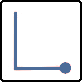
\includegraphics[angle=0,width=0.1\linewidth,keepaspectratio='true']{figures/dr.png}}] BD, escrevendo um “L”: mostra a lista de Waypoints 
\item[\raisebox{-1em}
{
\includegraphics[angle=0,width=0.1\linewidth,keepaspectratio='true']{figures/rd.png}}] DB, escrevendo um “T”: abre o gerenciador de provas
\item[\raisebox{-1em}
{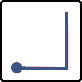
\includegraphics[angle=0,width=0.1\linewidth,keepaspectratio='true']{figures/dl.png}}] BE: mostra a lista alternativa
\item[\raisebox{-1em}
{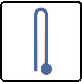
\includegraphics[angle=0,width=0.1\linewidth,keepaspectratio='true']{figures/ud.png}}]CB: ativa o Auto Zoom
\end{itemize}
\vspace{2em}

\subsection*{Gestos sofisticados:}
\begin{itemize}
\item[\raisebox{-1em}
{
\includegraphics[angle=0,width=0.1\linewidth,keepaspectratio='true']{figures/urd.png}}] CDB, escrevendo um “A”: mostra janela de análises
\item[\raisebox{-1em}
{
\includegraphics[angle=0,width=0.1\linewidth,keepaspectratio='true']{figures/ldrdl.png}}]EBDBE, escrevendo um “S”: mostra a janela de Estado. 
\end{itemize}
